\section{Introduction}
\label{sec:intro}


Recent work has explored the potential of using large language models (LLMs) as assistants in creative writing tasks, from stories to screenplays 
\cite{mirowski2023cowriting,yang2022re3,lee2022coauthor,ippolito2022creative,chen2023ambient}. An important aspect of this research is to investigate LLMs’ capabilities in terms of their ability to both \textit{generate} creative content and \textit{assess} whether a piece of writing is creative, with the ultimate goal of informing interaction design. However, evaluating objectively the creativity of a piece of writing is challenging. 

We propose a protocol to evaluate \textit{creativity as product} grounded in a widely accepted protocol that evaluates \textit{creativity as process} --- the Torrance Tests of Creative Thinking (TTCT) \cite{torrance1966torrance}. Based on Guilford's work on divergent thinking \cite{guilford1967nature}, TTCT measures creativity as a process by testing participants’ abilities in dealing with unusual uses of objects, specific situations, or impossibilities. TTCT is centered around evaluating four dimensions of creativity: \textit{fluency} (the sheer volume of meaningful ideas produced in reaction to a given stimulus), \textit{flexibility} (the diversity of categories within the responses), \textit{originality} (the uniqueness or novelty of answers) and \textit{elaboration} (the depth or granularity of details within the responses). 
While the direct application of TTCT might not be possible across diverse creative domains \cite{amabile1982social,baer2009assessing}, its four fundamental dimensions have proven adaptable \cite{trisnayanti2019development,mcintyre2003individual,10.1145/3313831.3376495}. Thus, based on TTCT and using the Consensual Assessment Technique (CAT) \cite{amabile1982social} we design the \textit{Torrance Tests for Creative Writing (TTCW)} to evaluate \textit{creativity as product} (Section \ref{design} Design Principle 1 and 2; Figure \ref{pipeline} Step 1). %SM-rr I added Step 1
The Consensual Assessment Technique states that the most valid assessment of the creativity of an idea or creation in any field is the collective judgment of experts in that field. Thus, to design TTCW, we asked 8 creative writing experts in a formative study (Section~\ref{sec:approach}) to propose creativity measures for the evaluation of short fictional stories aligned with the four Torrance dimensions. This resulted in 14 binary tests organized across the four original Torrance dimensions of \textit{fluency, flexibility, originality} and \textit{elaboration} (Section~\ref{CreativityTest}). 

\begin{figure*}
\centering
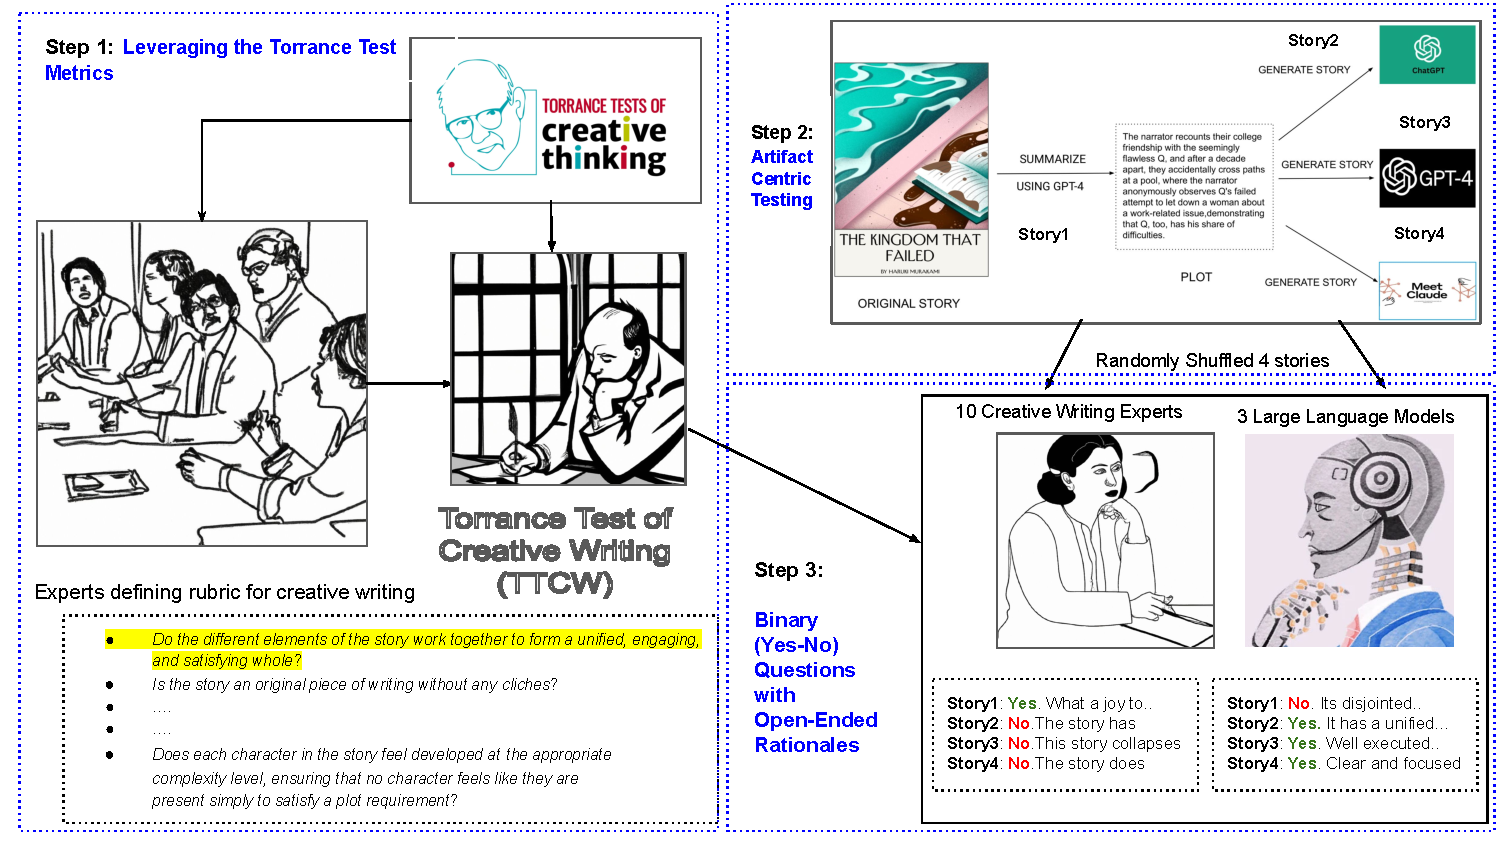
\includegraphics[width=\textwidth]{figures/CHI_pipeline.pdf}
\caption{\label{pipeline}Pipeline showing the construction of TTCW and evaluation of short stories using the TTCW framework where Step 1) shows how experts leverage the process-oriented Torrance Test of Creative Thinking to create 14 tests for evaluating creativity in short stories as a product. Step 2) demonstrates artifact-centric testing where 4 stories based on a single plot are used as a product of creativity evaluation Step3) shows an evaluation of stories using the TTCW framework by both expert humans and LLMs where they each provide Yes/No answers to individual tests followed by natural language rationales justifying their decision.}
\end{figure*}

To empirically validate TTCW as an evaluation protocol for creativity as product (fictional short stories), we build a benchmark consisting of 48 short stories: 12 stories written by professionals, and 36 by three top performing LLMs (ChatGPT \cite{ChatGPT}, GPT4 \cite{OpenAI2023GPT4TR} and Claude 1.3 \cite{Claude}) with 1400 words on average per story (Section~\ref{sec:data}; Figure \ref{pipeline} Step 2). %SM-rr I added Step 2
We recruit a new set of 10 experts, again adhering to CAT, to administer the 14 tests of TTCW on each story, collecting 3 evaluations per story. In this \textit{TTCW implementation with experts as assessors} (Figure \ref{pipeline} Step 3) %SM-rr I added Step 3
we aim to answer three research questions: 
\begin{enumerate}[label=RQ\arabic*:,leftmargin=3em]
     \item \textit{Is the TTCW-based creative evaluation consistent and reproducible? In other words, is there agreement among expert annotators when they perform tests on the same stories?} Based on a total of 2,000+ expert-administered tests, our findings reveal that experts reach moderate agreement on average (Fleiss Kappa 0.41) across the 14 TTCW tests, and reach strong agreement when considering the aggregated tests (Pearson correlation $0.69$). This confirms the validity of TTCW for the evaluation of creativity in fictional short stories.\\
     
    \item \textit{Are the human-written stories more likely to pass individual TTCW than LLM-generated stories? If so, which tests demonstrate the most significant gaps?} The analysis of the conducted tests reveals that the 12 expert-written stories pass an average of 84.7\% of the tests, confirming that although an expert story must not pass all tests to be deemed creative, experienced writers typically produce artifacts that pass the majority of the tests. In comparison, LLM-generated stories pass many fewer tests on average, from 9\% for ChatGPT-generated stories, up to 30\% for Claude-generated stories. In other words, LLM-generated stories are three to ten times less likely to pass individual TTCW tests compared to expert-written stories, revealing a wide gap in the evaluated creativity of LLM-generated content.\\ 
    
    \item \textit{Which LLMs perform better in TTCW evaluation, and are there specializations observed, with some different LLMs performing better on different Torrance dimensions?} Besides the general gap, the granularity of the TTCW reveals that individual LLMs differ in abilities, with GPT4 more likely to pass tests associated with Originality, and Claude V1.3 more likely to pass tests in Fluency, Flexibility and Elaboration.
\end{enumerate}

Prior work \cite{ippolito2022creative} has argued that given the nature of LLMs where they regurgitate text seen during pre-training, they are often unable to directly generate a truly original and creative piece of writing (Also see Section \ref{expertvsai}). However, they might be utilized in providing feedback to authors during their writing process \cite{chakrabarty2023creativity}. Thus, we perform a study of \textit{TTCW implementation with LLMs as assessors} (Section ~\ref{sec:llmeval}; and Figure \ref{pipeline} Step 3) %SM-rr I added Step 3
to understand whether LLMs can be used to assess creative writing. 
We expanded each test into a detailed prompt, and measured whether LLM assessments correlate with collected expert judgments. Our analysis reveals that for the most part, LLMs are not capable of administering the TTCW tests, as the three LLMs we experiment with achieve correlations with experts that are close to zero.

In summary, our work makes the following contributions:
\begin{itemize}
    \item We adapt the Torrance Test for Creative Thinking (TTCT), a protocol for evaluating creativity as a process, and align it for the evaluation of creativity as a product particularly focusing on short stories. Using the Consensual Assessment Technique, we design 14 tests called the \textit{Torrance Test for Creative Writing (TTCW)} based on the four original Torrance dimensions of fluency, flexibility, originality, and elaboration,
    \item We experimentally validate the TTCW through an assessment of 48 stories involving 10 participants with expertise in creative writing, finding that they reach moderate agreement when administering individual tests, and strong agreement when evaluating all tests in aggregate.
    \item We study the abilities of LLMs to generate stories that pass/fail the TTCW tests and their ability to reliably assess the creativity of stories following the TTCW framework through correlation with human judgments. Our findings show that LLM-generated stories are three to ten times less likely to pass TTCW tests compared to expert-written stories, as well as the fact that current state-of-the-art LLMs are not yet capable of reproducing expert assessments when administering TTCW tests. To enable future research in this fast-evolving domain, we release the large-scale annotation of 2,000+ TTCW assessments, each accompanied with a natural language expert explanation. 
    \item Finally, we discuss how creative writing experts can distinguish between AI vs. human written stories and how future work can use our evaluation framework for building rich interactive writing support tools.
\end{itemize}
